\documentclass[final]{beamer}

% Beamer poster
\mode<presentation>{\usetheme{icassp2019}}
\usepackage[orientation=landscape,size=a0,scale=1.31]{beamerposter}
\setbeamertemplate{itemize subitem}{\mybf{--}}
% \setbeamertemplate{itemize subitem}{\raisebox{0.12ex}{$\blacktriangleright$}\hskip0.1em}
\definecolor{tablue20blue}{RGB}{31,119,180}
\definecolor{tablue20orange}{RGB}{255,127,14}
\definecolor{tablue20red}{RGB}{214,39,40}
\definecolor{tablue20green}{HTML}{2ca02c}
\newcommand{\nonparallel}[1]{\textcolor{tablue20orange}{#1}}
\newcommand{\goal}[1]{\textcolor{tablue20orange}{#1}}
\newcommand{\zeroshot}[1]{\textcolor{tablue20blue}{#1}}
\newcommand{\realtime}[1]{\textcolor{tablue20red}{#1}}
\newcommand{\highqual}[1]{\textcolor{tablue20green}{#1}}

\definecolor{softgreen}{RGB}{25, 168, 34}
\definecolor{softred}{RGB}{188, 26, 11}

\usepackage{booktabs}
\usepackage{tabularx}
\usepackage{multirow}

\newcommand{\mytable}{
    \centering
    \small
    \renewcommand{\arraystretch}{1.2}
    }
\renewcommand{\tabularxcolumn}[1]{m{#1}}
\newcolumntype{C}{>{\centering\arraybackslash}X}
\newcolumntype{L}{>{\raggedright\arraybackslash}X}
\newcolumntype{R}{>{\raggedleft\arraybackslash}X}
\newcolumntype{P}[1]{>{\raggedright\arraybackslash}p{#1}}
\usepackage{siunitx}
\sisetup{detect-all}
\usepackage{etoolbox}                           % bold fonts in table
\newcommand{\ubold}{\fontseries{b}\selectfont}  % bold fonts in table
\robustify\ubold                                % bold fonts in table
\newcommand{\tablecaptionsep}{\vspace*{-0pt}}

% Graphics
\graphicspath{{fig/}}

% Mathematics
\usefonttheme[onlymath]{serif}
% \usefonttheme{serif}
\renewcommand{\vec}[1]{\boldsymbol{\mathbf{#1}}}

% Colours
\newcommand{\graybf}[1]{\textcolor{darkestgray}{\textbf{#1}}}
% \newcommand{\mybf}[1]{\textbf{#1}}
\newcommand{\mybf}[1]{\textcolor{darkestgray}{\textbf{#1}}}

% Layout
\newlength{\columnheight}
% \setlength{\columnheight}{66.25cm} % landscape
\setlength{\columnheight}{66.25cm} % landscape
% \setlength{\columnheight}{65.5cm} % landscape
% \setlength{\columnheight}{103cm} % portrait

% Tables
\usepackage{booktabs}
\usepackage{tabularx}
% \newcommand{\mytable}{\centering
                    %   \renewcommand{\arraystretch}{1.05}
                    %   }
\newcolumntype{C}{>{\centering\arraybackslash}X}
\newcolumntype{L}{>{\raggedright\arraybackslash}X}
\newcolumntype{R}{>{\raggedleft\arraybackslash}X}
\renewcommand{\tabularxcolumn}[1]{m{#1}}

% Text
\newcommand{\system}[1]{{\footnotesize \textsc{#1}}}

% Title and author
\title{A Temporal Extension of \\Latent Dirichlet Allocation for \\Unsupervised Acoustic Unit Discovery}
\author{Werner van der Merwe, Herman Kamper, Johan du Preez}
\institute{MediaLab, E\&E Engineering, Stellenbosch University, South Africa}

\begin{document}

\begin{frame}[t]
    \begin{columns}[T]

        \begin{column}{.01\linewidth}\end{column} % border column


        \begin{column}{.33\linewidth}
            \centering
            \begin{minipage}[T]{.97\textwidth}\parbox[t][\columnheight]{\textwidth}{

                    % ================================
                    %  BACKGROUND BLOCK
                    % ================================
                    \begin{block}{Unsupervised acoustic unit discovery}

                        \begin{itemize}
                            \vspace{-0.5cm}
                            \setlength{\itemsep}{0.5ex}
                            \item Annotating speech is often not possible for many low-resource languages. 
                            \item Unsupervised acoustic unit discovery (AUD)  aims to solve this by finding a set of phone-like units from speech that resembles the phonetic inventory of a language.
                        \end{itemize}

                    \end{block}

                    % ================================
                    %  COMPONENTS OF VC SYSTEMS
                    % ================================
                    \begin{block}{Vector-quantised neural networks}

                        \begin{itemize}
                            \vspace{-0.5cm}
                            \setlength{\itemsep}{0.5ex}
                            \item Recently vector-quantised (VQ) neural networks such as the variational autoencoder (VQ-VAE) and contrastive predictive coding (VQ-CPC) have performed well in unsupervised AUD\@.
                            \item Despite good performance, the number of VQ codes in these models (512 for the VQ model in this paper)
                                  is often far more than the number of true phone units used in a language (in the order of 50).
                            \item To more closely match the phonetic inventory of a language, the larger set of VQ codes therefore need to be mapped to a smaller set.
                        \end{itemize}


                        \begin{figure}[t]\label{fig:aud_example}
                            \centering
                            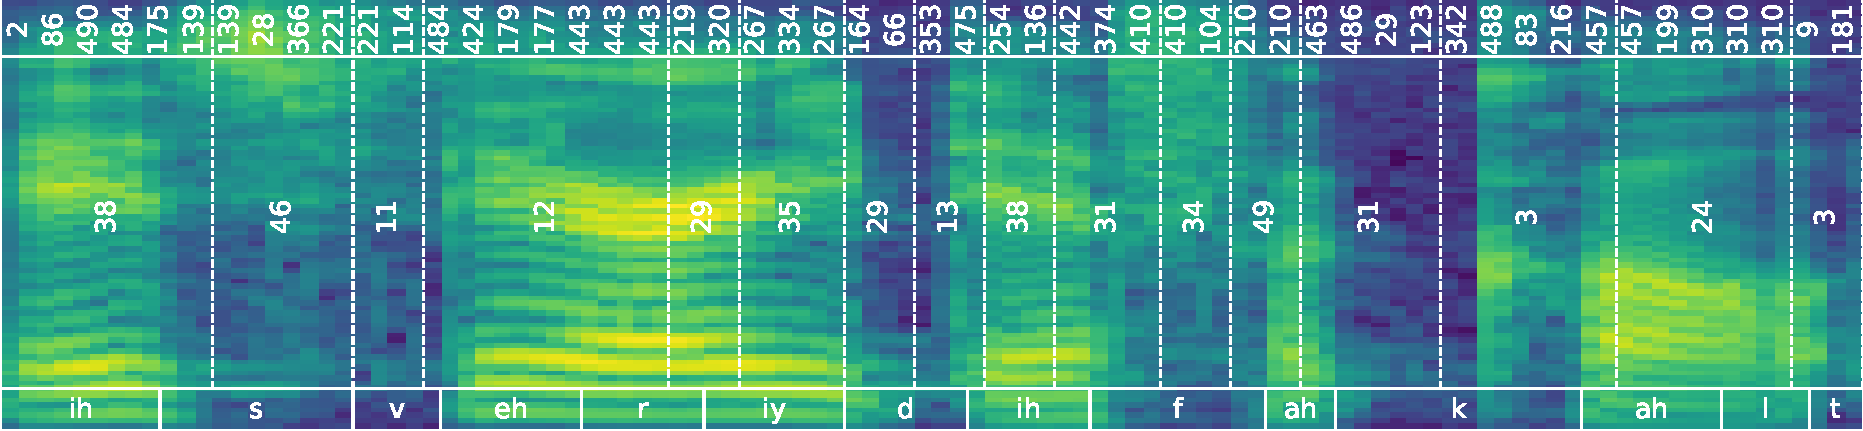
\includegraphics[width=\linewidth]{figures/aud_example}
                            \caption[Acoustic unit discovery of an utterance]{
                                This figure gives a spectrogram of the spoken utterance, ``Is very difficult''.
                                The labels on the figure from top to bottom are from a VQ-VAE, Markov chain latent Dirichlet allocation (MCLDA) and a professional transcriber.}
                        \end{figure}

                    \end{block}

                    % ================================
                    %  Latent Dirichlet allocation
                    % ================================
                    \begin{block}{Latent Dirichlet allocation}

                        \begin{itemize}
                            \vspace{-0.5cm}
                            \setlength{\itemsep}{0.5ex}
                            \item Latent Dirichlet allocation (LDA) is widely used for unsupervised topic modelling on sets of documents.
                            \item The LDA model is a parametric bag-of-VQ-codes model and considers no temporal information. 
                        \end{itemize}

                        \vspace{-0.5cm}
                        \begin{figure}[t]
                            \centering
                            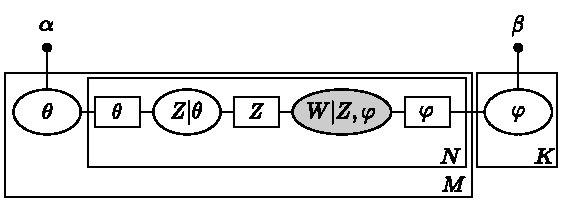
\includegraphics[width=\linewidth]{figures/base_lda}
                            \caption{The cluster graph of latent Dirichlet allocation model.}
                            \label{fig:base_lda}
                        \end{figure}

                    \end{block}

                }\end{minipage}
        \end{column}



        \begin{column}{.33\linewidth}
            \centering
            \begin{minipage}[T]{.97\textwidth}\parbox[t][\columnheight]{\textwidth}{

                    % ================================
                    %  Markov chain latent Dirichlet allocation
                    % ================================
                    \begin{block}{Markov chain latent Dirichlet allocation}

                        \begin{itemize}
                            \vspace{-0.5cm}
                            \setlength{\itemsep}{0.5ex}
                            \item We extend LDA to include a Markov chain between adjacent phone units to model transitions.
                            \item With this model we introduce the scaler parameter $a$ to increase the probability of repeating phone-like units.
                            $$
                            \setlength\itemsep{0em}
                            p(\bm{Z}_n,\bm{Z}_{n-1}) =
                            \begin{cases}
                              \frac{a}{K^2 + K(a-1)}, & Z_n = Z_{n-1}    \\
                              \frac{1}{K^2 + K(a-1)}, & Z_n \neq Z_{n-1}
                            \end{cases}
                            \label{eq:transition_probability}
                         $$
                            \end{itemize}

                        \vspace{-0.5cm}
                        \begin{figure}[t]
                            \centering
                            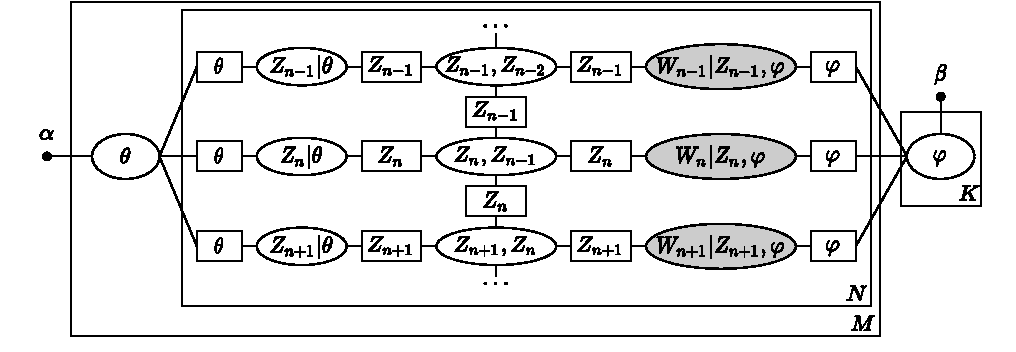
\includegraphics[width=\linewidth]{figures/werner_lda}
                            \caption{The cluster graph of Markov chain latent Dirichlet allocation model.}
                            \label{fig:base_lda}
                        \end{figure}

                    \end{block}

                    \begin{block}{Experimental setup}

                        \begin{itemize}
                            \vspace{-0.5cm}
                            \setlength{\itemsep}{0.5ex}
                            \item A VQ-VAE model is used to extract utterances with 512 VQ codes from the Buckeye speech corpus.
                            \item The Markov chain LDA model uses these VQ codes to discover 50 latent phone-like units.
                            \item We compare the base LDA and expanded Markov chain LDA to an established CPC-Big + \(K\)-means model that clusters CPC representations directly into 50 units.

                        \end{itemize}
                    \end{block}

                    % ================================
                    %  Metrics
                    % ================================
                    \begin{block}{Metrics} % {\large (\%)}}

                        \begin{itemize}
                            \vspace{-0.4ex}
                            \setlength{\itemsep}{0.5ex}
                            \item We compare the output of models to the ground truth transcriptions in terms of phone segmentation and cluster quality.
                        \end{itemize}

                        \begin{figure}[!t]
                            \centering
                            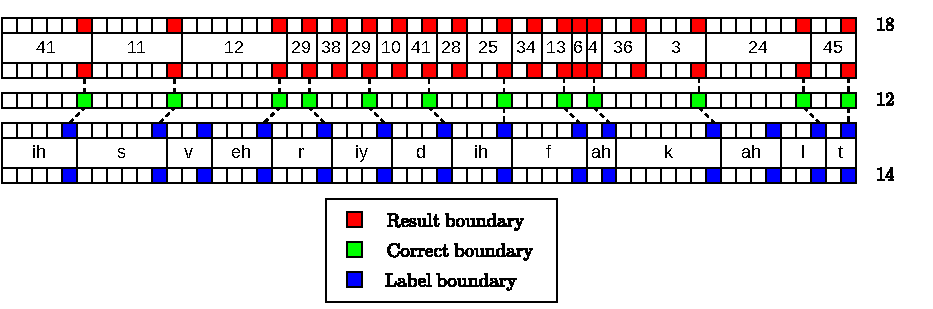
\includegraphics[width=0.95\linewidth]{figures/phone_boundaries}
                            \caption[Phone boundary example]{
                                The following figure illustrates how to determine if a phone boundary is correct.
                            }
                            \label{fig:phone_boundaries}
                        \end{figure}
                    \end{block}


                }\end{minipage}
        \end{column}



        \begin{column}{.33\linewidth}
            \centering
            \begin{minipage}[T]{.97\textwidth}\parbox[t][\columnheight]{\textwidth}{

                    % ================================
                    %  Results: Phone Segmentation
                    % ================================
                    \begin{block}{Results: Phone Segmentation}
                        % Extent to which each model satisfies the four practicality requirement:

                            \vspace{-0.5ex}

                        \begin{table}[!t]
                            \caption{Phone segmentation results (\%) on Buckeye speech test.
                            100\% in all metrics would be perfect segmentation. 
                            Negative R-value}
                            \mytable
                            \centering
                            %  \begin{tabularx}{\linewidth}{@{} lllll @{}}
                            \begin{tabularx}{\linewidth}{@{}lRRRR@{}}
                                \toprule
                                Model            & \textit{Precision}         & \textit{Recall}         & \textit{F-score}       & \textit{R-value}         \\
                                \midrule
                                \multicolumn{2}{@{}l}{\underline{\textit{Speaker dependent}}}                        \\
                                CPC-Big + km-50  & $35.3$      & $94.0$      & $51.3$      & $-44.4$                 \\
                                VQ-VAE           & $32.1$      & $\bm{97.6}$ & $48.1$      & $-80.7$                 \\
                                LDA              & $36.0$      & $94.9$      & $52.00$     & $-45.0$                 \\
                                Markov chain LDA & $\bm{55.1}$ & $72.4$      & $\bm{62.2}$ & $\hphantom{-}\bm{55.6}$ \\
                                \addlinespace
                                \multicolumn{2}{@{}l}{\underline{\textit{Speaker independent}}}                      \\
                                CPC-Big + km-50  & $35.5$      & $93.9$      & $51.6$      & $-42.5$                 \\
                                VQ-VAE           & $32.0$      & $\bm{97.7}$ & $48.2$      & $-76.2$                 \\
                                LDA              & $36.8$      & $93.3$      & $52.8$      & $-33.4$                 \\
                                Markov chain LDA & $\bm{55.4}$ & $66.4$      & $\bm{60.4}$ & $\hphantom{-}\bm{61.6}$ \\
                                \bottomrule
                            \end{tabularx}
                            \label{tab:seg_results}
                        \end{table}

                    \end{block}

                    % ================================
                    %  Results: Cluster quality
                    % ================================
                    \begin{block}{Results: Cluster quality}
                        \vspace{-0.5ex}
                        \begin{table}[!t]
                            \caption{Clustering quality results (\%) on Buckeye speech test set.
                            The desired purity and mutual information is 100\% while a lower singleton \% is better.}
                            \centering
                            \mytable
                            \begin{tabularx}{\linewidth}{@{}  lRRR @{}}
                                \toprule

                                {Model}          & \textit{Cluster Purity}    & \textit{Singletons}                & \textit{Mutual Information}       \\
                                \midrule
                                \multicolumn{2}{@{}l}{\underline{\textit{Speaker dependent}}}              \\
                                CPC-Big + km-50  & $33.1$      & $\hphantom{1}9.3$           & $\bm{39.6}$ \\
                                VQ-VAE           & $\bm{34.0}$ & $26.7$                      & $38.4$      \\
                                LDA              & $24.1$      & $20.2$                      & $26.6$      \\
                                Markov chain LDA & $29.1$      & $\hphantom{\bm{.}}\bm{4.5}$ & $30.6$      \\
                                \addlinespace
                                \multicolumn{2}{@{}l}{\underline{\textit{Speaker independent}}}            \\
                                CPC-Big + km-50  & $\bm{32.3}$ & $\hphantom{1}9.3$           & $\bm{37.8}$ \\
                                VQ-VAE           & $31.8$      & $27.0$                      & $34.3$      \\
                                LDA              & $21.5$      & $18.9$                      & $22.0$      \\
                                Markov chain LDA & $27.3$      & $\hphantom{\bm{.}}\bm{4.0}$ & $24.7$      \\
                                \bottomrule
                            \end{tabularx}
                            \label{tab:cluster_results}
                        \end{table}

                 \end{block}

                    % \vfill
                    % ================================
                    % Conclusions
                    % ================================
                    \begin{block}{Conclusions}
                        % \vspace{-0.0ex}
                        \begin{itemize}
                            % \vspace{-0.5cm}
                            \setlength{\itemsep}{0.5ex}
                            \item We have shown that the inclusion of temporal information in an LDA model increases the AUD phone segmentation and mutual information.
                            \item The Markov chain LDA achieved better phone segmentation results than the base LDA and the CPC-Big +  $K$-means method.
                            \item The mutual information from our Markov chain LDA model was lower than that of the CPC-Big + \(K\)-means method we compared against, but achieved better phone segmentation results.
                            \item The introduction of more informative priors could result in an increased mutual information.

                        \end{itemize}

                    \end{block}



                }\end{minipage}
        \end{column}



        \begin{column}{.01\linewidth}\end{column} % border column

    \end{columns}
\end{frame}

\end{document}